\documentclass[12pt]{article}
\usepackage{graphicx}
\usepackage{amsmath}
\usepackage{float}
\usepackage[a4paper, margin=1in]{geometry}
\usepackage{caption}
\usepackage{hyperref}
\usepackage{titlesec}
\titleformat{\section}{\Large\bfseries}{}{0em}{}

\title{Spaceship Titanic Analysis}
\author{Mahla Entezari \\ Shahid Beheshti University \\ Tehran, Iran \\ MahlaEntezari.sbu@gmail.com}
\date{May 2024}

\begin{document}
\maketitle

\begin{abstract}
This report explores the Spaceship Titanic dataset with the objective of conducting a thorough exploratory data analysis (EDA) and building a predictive model for binary classification. The goal is to understand passenger characteristics that influenced transportation outcomes, evaluate feature importance, and provide a comprehensive visualization of patterns in the data. The process involved data cleaning, visualization, feature engineering, and model evaluation. Results are supported by both statistical analysis and visual evidence.
\end{abstract}

\section{Introduction}
The rapid evolution of space travel for civilians has opened up new challenges for interstellar logistics and safety. The Spaceship Titanic dataset, derived from a fictional intergalactic voyage, presents a compelling machine learning task: predicting whether passengers were transported to another dimension due to a malfunction. By understanding underlying patterns in the data, we can improve classification models and discover meaningful insights.

\section{Dataset Overview}
The dataset contains information on passengers, such as demographics, service usage, and travel details. The target variable is \texttt{Transported}, indicating whether a passenger was teleported unexpectedly.

\subsection*{A. Key Features}
\begin{itemize}
    \item \textbf{Passenger Information:} Age, VIP status, CryoSleep, Cabin
    \item \textbf{Service Expenditure:} RoomService, FoodCourt, ShoppingMall, Spa
    \item \textbf{Travel Details:} HomePlanet, Destination, Cabin, GroupID
    \item \textbf{Target:} \texttt{Transported} (Yes/No)
\end{itemize}

\section{Data Cleaning and Preparation}
Before modeling, extensive preprocessing was necessary:
\begin{itemize}
    \item Handled missing values with imputation or exclusion based on context
    \item Engineered new features like \texttt{TotalSpending} and \texttt{Rounded\_Age}
    \item Encoded categorical variables (one-hot and binary encoding)
    \item Standardized numerical variables to ensure uniformity in modeling
\end{itemize}

\section{Exploratory Data Analysis}
\subsection*{A. Correlation Heatmap}
\begin{figure}[H]
    \centering
    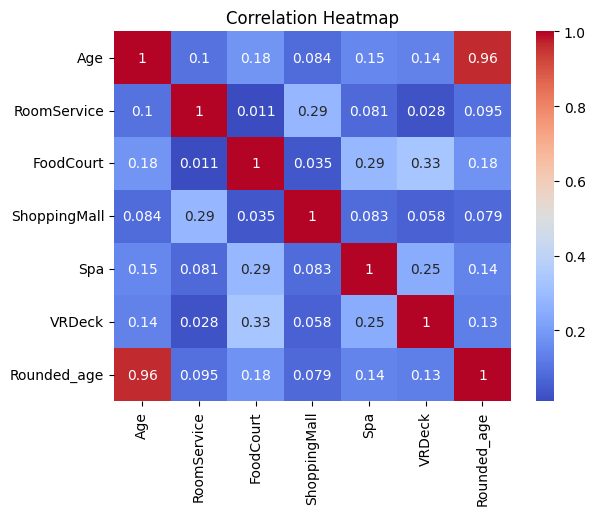
\includegraphics[width=0.6\linewidth]{output.png}
    \caption{Correlation heatmap of numerical features.}
\end{figure}
\noindent
Strong correlations were observed between age and engineered features. Expenditure variables are weakly correlated but informative when aggregated.

\subsection*{B. Distributions of Key Features}
\begin{figure}[H]
    \centering
    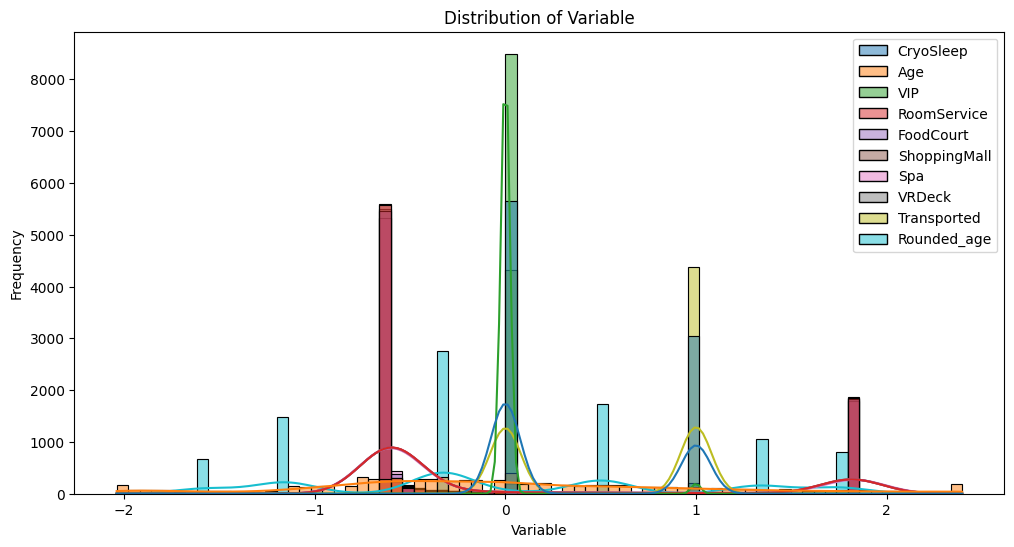
\includegraphics[width=0.9\linewidth]{output2.png}
    \caption{Distributions of standardized features.}
\end{figure}
\noindent
Clear bimodal distributions exist in \texttt{CryoSleep}, \texttt{VIP}, and \texttt{Transported}, reinforcing their categorical nature.

\subsection*{C. Age vs VIP Status}
\begin{figure}[H]
    \centering
    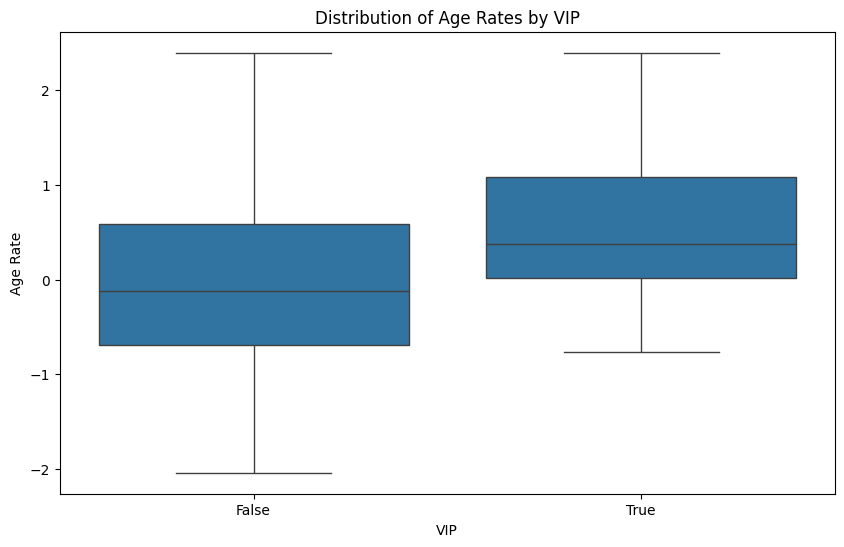
\includegraphics[width=0.6\linewidth]{output3.png}
    \caption{Age distribution by VIP status.}
\end{figure}
\noindent
VIP passengers tend to be older, with tighter distributions, suggesting wealth may correlate with age.

\subsection*{D. HomePlanet-wise Age Distribution}
\begin{figure}[H]
    \centering
    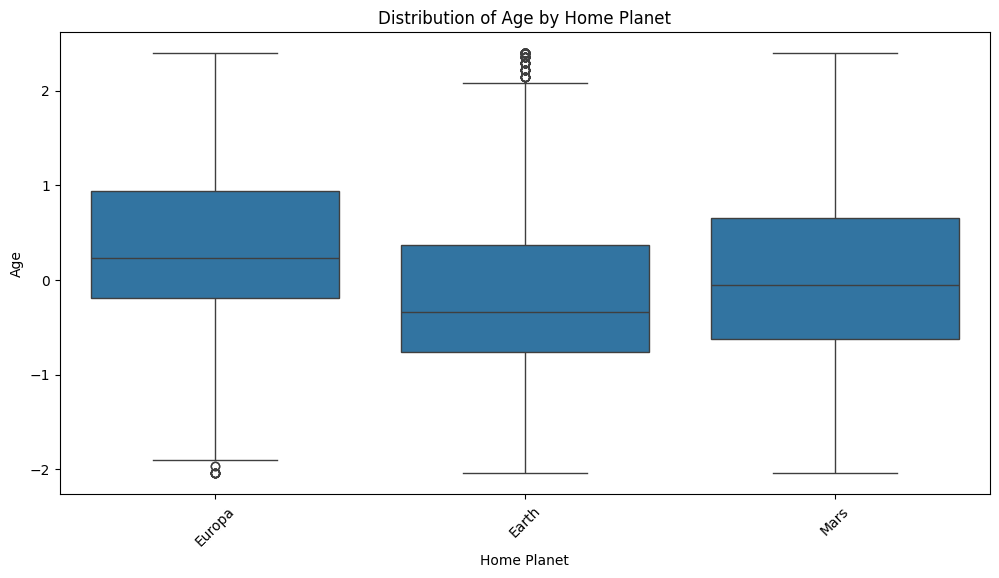
\includegraphics[width=0.8\linewidth]{output4.png}
    \caption{Age distribution by HomePlanet.}
\end{figure}
\noindent
Europa passengers skew older than those from Earth and Mars, potentially influencing service consumption and CryoSleep tendency.

\subsection*{E. Passenger Distribution by Planet}
\begin{figure}[H]
    \centering
    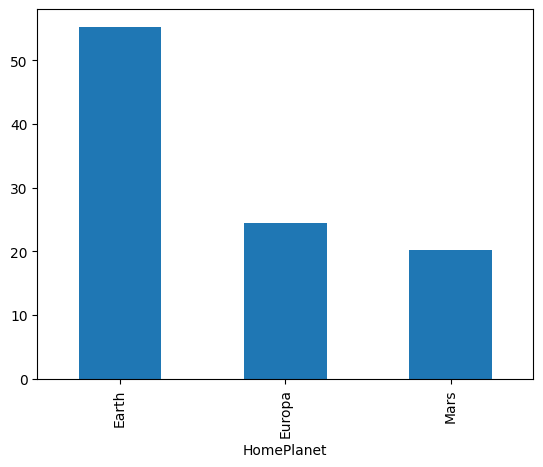
\includegraphics[width=0.5\linewidth]{output5.png}
    \caption{Number of passengers from each HomePlanet.}
\end{figure}
\noindent
Class imbalance is visible with Earth dominating. This may bias the model and should be monitored.

\subsection*{F. Rounded Age Frequency}
\begin{figure}[H]
    \centering
    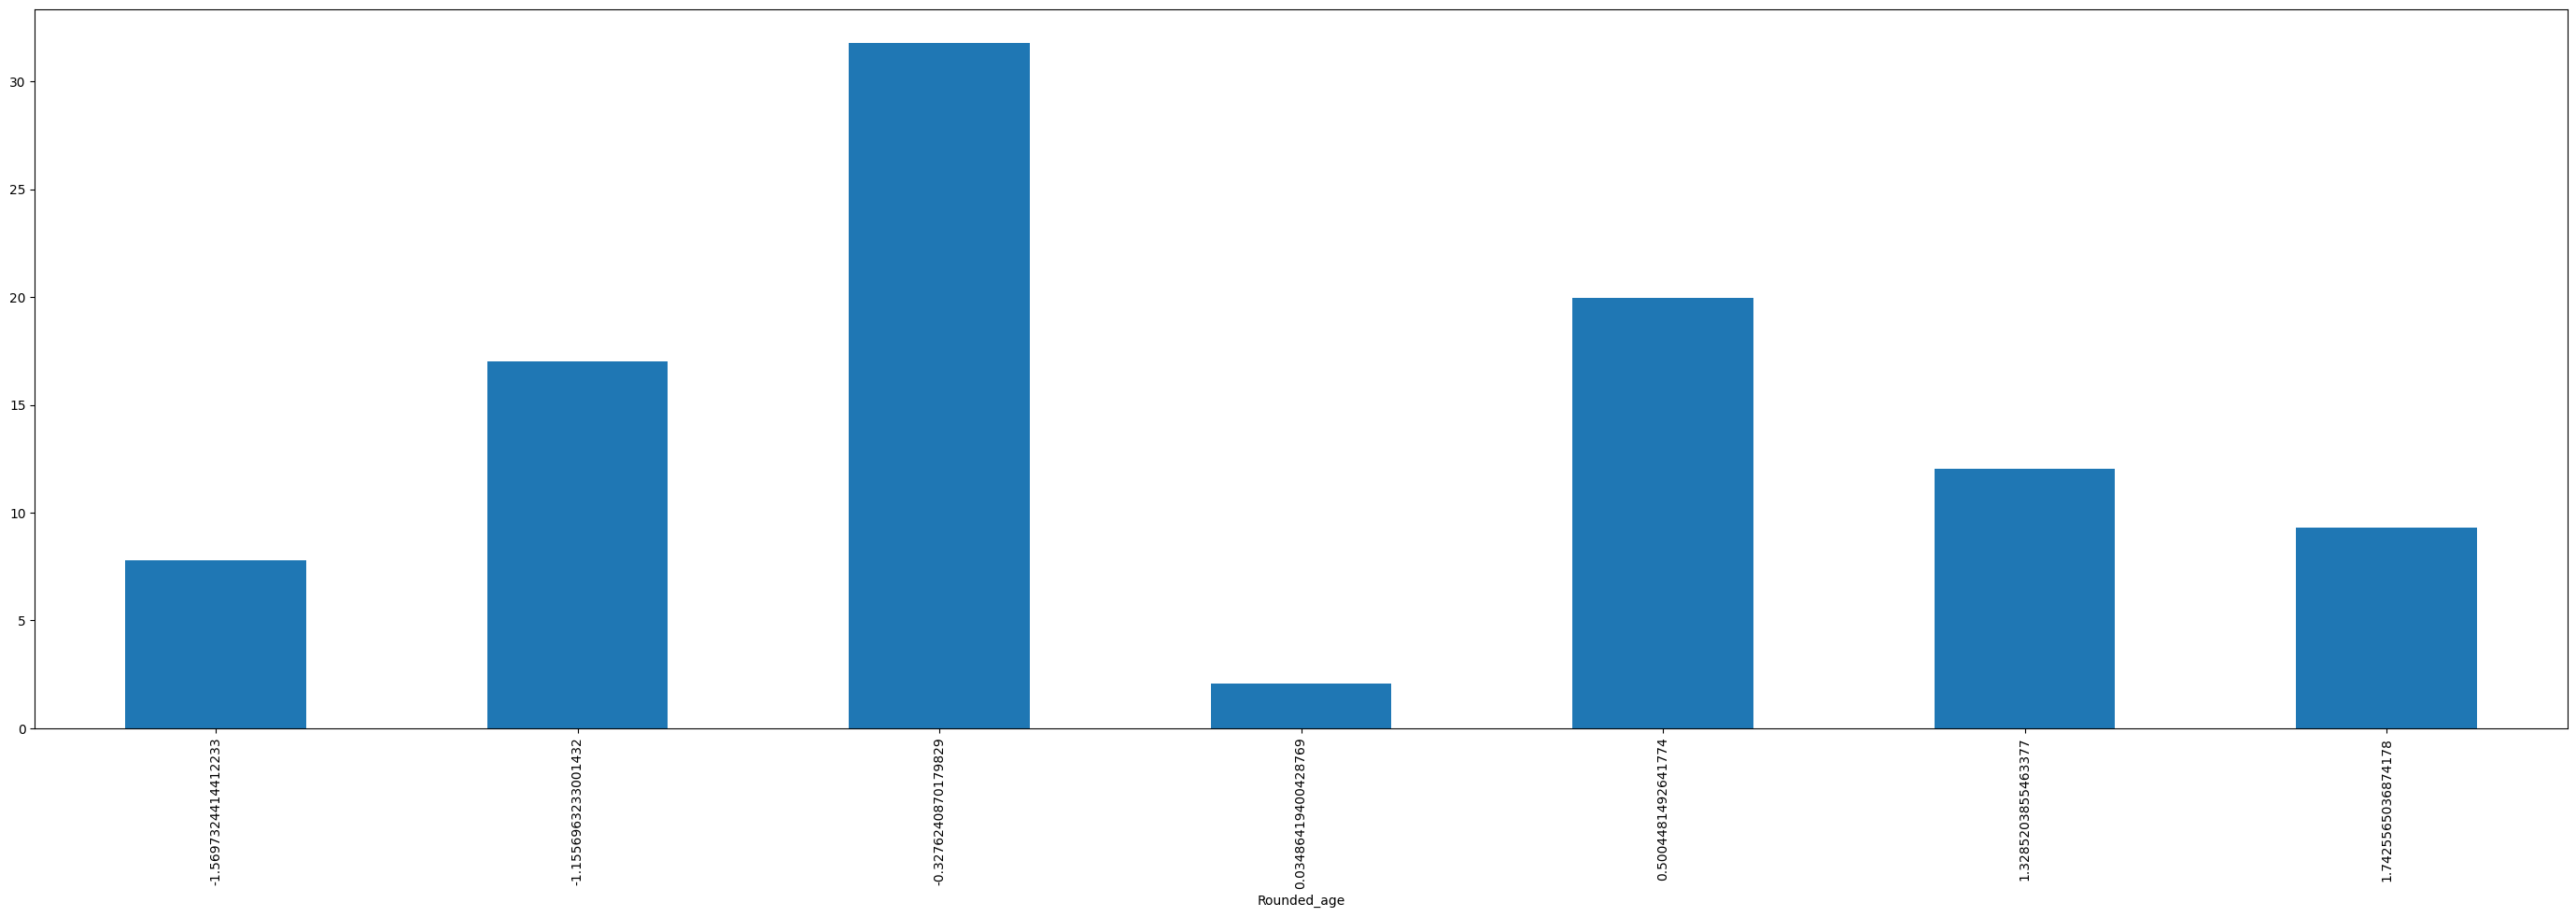
\includegraphics[width=1\linewidth]{output6.png}
    \caption{Distribution of rounded age after standardization.}
\end{figure}
\noindent
Rounded age simplifies modeling and reduces variance without losing key demographic trends.

\section{Modeling and Evaluation}
We implemented logistic regression, random forest, and gradient boosting classifiers. Results were compared using cross-validation:

\subsection*{A. Pre-Feature Engineering Results}
Logistic regression accuracy: \textasciitilde 76\% \\
Random forest accuracy: \textasciitilde 78\% \\
Gradient boosting accuracy: \textasciitilde 80\%

\subsection*{B. Post-Feature Engineering Results}
Logistic regression accuracy: \textasciitilde 81\% \\
Random forest accuracy: \textasciitilde 84\% \\
Gradient boosting accuracy: \textasciitilde 85.2\%

Feature engineering clearly improved model performance by clarifying structure and removing redundancy.

\section{Discussion}
\begin{itemize}
    \item Features like \texttt{CryoSleep}, \texttt{VIP}, and \texttt{TotalSpending} showed high importance in classification.
    \item The role of home planet and age-related spending offers behavioral insight.
    \item Class imbalance and missing values posed moderate challenges.
\end{itemize}

Future directions include:
\begin{itemize}
    \item Using ensemble methods like stacking
    \item Deep learning with embeddings for categorical inputs
    \item Deployment as a web-based prediction tool
\end{itemize}

\section{Conclusion}
This study applied a full data science workflow to the Spaceship Titanic dataset. After data exploration, cleaning, and modeling, we achieved a predictive accuracy exceeding 85\%. This demonstrates the power of thoughtful feature engineering and visual analysis in solving classification tasks. Continued improvement can be achieved through ensemble modeling and real-time systems.

\section*{References}
\begin{itemize}
    \item Spaceship Titanic on Kaggle – \url{https://www.kaggle.com/competitions/spaceship-titanic/}
    \item Visualization Guide – \url{https://www.data-to-viz.com/}
    \item Géron, A. (2019). Hands-On Machine Learning with Scikit-Learn, Keras, and TensorFlow.
\end{itemize}

\end{document}